% Chapter 17 - Amino Acids.tex
% Copyright (c) 2014 - 2016, zhiayang@gmail.com
% Licensed under the Apache License Version 2.0.

\pagebreak
\hypertarget{ChapterAminoAcids}{}
\part{Amino Acids}

	\section{Overview}

		Amino acids are the basic components of proteins, and are basically molecules containing \itl{both} an amine group, and a carboxylic
		group. More specifically, α-amino acids are amino acids where both the amine and carboxylic acid groups are attached to the same carbon.
		There is one always one hydrogen, and one R group.

		The 20 naturally-occurring α-amino acids have names and other stuff, and are reproduced in
		\hyperlink{AppendixListOfAminoAcids}{\boit{the appendix}}. The simplest α-amino acid is glycine, where the R-group is hydrogen (ie.
		there are two hydrogens attached to the central carbon).

		All other α-amino acids are chiral, as they have 4 distinct groups attached to the central carbon.

		\subsection{Acidic and Basic Amino Acids}

			Even though all amino acids have one \ch{-CO2H} group and one \ch{-NH2} group, they are, by default, considered \itl{neutral}. An
			amino acid is considered basic if there are one or more \ch{-NH2} groups along the R-group chain, and similarly considered
			acidic if there are one or more \ch{-CO2H} groups in the R-group.

		% end subsection

		\subsection{Polarity}

			The polar nature of an amino acid is determined by the nature of the R group, since the acid and base group on the backbone would
			cancel each others' dipoles.

			If the amino acid has R groups that can form hydrogen bonds or ion-dipole interactions, then it is a polar amino acid. Otherwise,
			if it contains for instance only alkyl groups, it is non-polar.

		% end subsection

	% end section


	\pagebreak
	\section{Zwitterions}

		Zwitterions are quite possibly one of the most ridiculous names ever created for anything. A zwitterion is an amino acid that is
		electrically neutral, ie. the \ch{-NH2} group is protonated into \ch{-NH3+}, and the \ch{-CO2H} group is deprotonated into \ch{-CO2-}.

		Amino acids undergo an \itl{intramolecular} acid-base reaction to form zwitterions.

		\diagram[1.0]{
			\schemestart[0,1.5,thick]
				\chemfig{C(-[:0]C(=[:60]!\molO)(-[:300]!\molOH))(-[:180]!\molN(-[:120]H)(-[:240]H))(-[:90]H)(-[:270]!\molR)}
				\arrow{<=>}
				\chemfig{C(-[:0]C(=[:60]!\molO)(-[:300]!\molO|\mchg))(-[:180]\pchg|{\color{RoyalBlue}N}(-[:90,,2]H)(-[:180,,2]H)(-[:270,,2]H))(-[:90]H)(-[:270]!\molR)}
			\schemestop
		}

		In aqueous mediums and in the solid form, amino acids exist as zwitterions. Hence they share many similarities in terms of physical
		properties with ionic solids, such as a relatively high melting point (in contrast with other organic molecules).


		\subsection{Physical Properties}

			Amino acids have rather high melting points, for instance glycine, the simplest α-amino acid, has a melting point of
			\SI{262}{\celsius}, which is due to the strong electrostatic attractions between the zwitterions.

			They are also very soluble in water, due to the ability to form favourable ion-dipole interactions with surrounding water
			molecules.

		% end subsection


		\subsection{Isoelectric Point}

			The \itl{isoelectric point}, or \pI{}, of an amino acid is the \pH{} at which the amino acid exists as a
			zwitterion. The nature of the side-chain dictates the isoelectric point.

			For the simplest amino acid glycine, the value of \pI{} is \num{6.01}, and it is a neutral amino acid since there are neither
			acidic nor basic groups in the side-chain. Note that the \pI{} is not \num{7}, because the electronegative \ch{N} atom
			increases the acidity of the \ch{CO2H} group, while the electronegativity of said group weakens the basicity of the \ch{NH2} group.

			For amino acids with basic groups in the side-chain, eg. lysine, the \pI{} is above \num{7}, in this case \num{9.74}, while for
			amino acids with acidic groups in the side chain, eg. aspartic acid, the \pI{} is below \num{7}, in this case \num{2.77}.

			At \pH{} levels below the isoelectric point, the amino acid exists mainly as cations, and will migrate towards the
			cathode (negative terminal). At \pH{} levels above the isoelectric point, the amino acid exists mainly as anions, and will
			migrate towards the positive anode.

		% end subsection


		\subsection{Acid-Base Behaviour}

			Since they have both acidic and basic groups, amino acids are \itl{amphoteric}, and their structure changes slightly depending
			on the \pH{} of the solution (mainly the \ch{H+} ions).

			\diagram[0.8]{
				\schemestart[0,1.5,thick]
					\chemname{\chemfig{C(-[:0]C(=[:60]!\molO)(-[:300]!\molOH))(-[:180]\pchg|{\color{RoyalBlue}N}(-[:90,,2]H)(-[:180,,2]H)(-[:270,,2]H))(-[:90]H)(-[:270]!\molR)}}{low \pH{}}
					\arrow{<=>[\ch{OH-}][\ch{H+}]}
					\chemname{\chemfig{C(-[:0]C(=[:60]!\molO)(-[:300]!\molO|\mchg))(-[:180]\pchg|{\color{RoyalBlue}N}(-[:90,,2]H)(-[:180,,2]H)(-[:270,,2]H))(-[:90]H)(-[:270]!\molR)}}{isoelectric \pH{}}
					\arrow{<=>[\ch{OH-}][\ch{H+}]}
					\chemname{\chemfig{C(-[:0]C(=[:60]!\molO)(-[:300]!\molO|\mchg))(-[:180]!\molN(-[:120]H)(-[:240]H))(-[:90]H)(-[:270]!\molR)}}{high \pH{}}
				\schemestop
			}

			At low \pH{} levels,, [\ch{H+}] in the solution is high. Thus, both the acid and base groups will be \itl{protonated}, resulting in a
			cation. Note that any acidic or basic groups in the side-chain will be protonated as well.

			At the isoelectric \pH{}, the amino acid exists as the zwitterion, where the acid group is deprotonated and the basic group remains
			protonated.

			At high \pH{} levels, [\ch{OH-}] in the solution is high, so all the relevant groups will be \itl{deprotonated}, leaving \ch{-CO2-} and
			\ch{-NH2}. Again, acidic or basic groups in the side-chain will be deprotonated as well.

		% end subsection

	% end section



	\section{Electrophoresis}

		Electrophoresis allows one to separate amino acids by way of their different isoelectric points. To conduct this electrophoresis, the
		mixture of amino acids to be separated is placed on a strip of filter paper, wet with a buffer solution at a certain \pH{}. The
		filter paper is then connected to an external source of voltage.

		Depending on the \pH{} of the buffer, the amino acids in the mixture will exist either as anions, cations, or zwitterions. These
		ions will then migrate to either the positive anode or the negative cathode, or stay put in the case of zwitterions.

		The distance of migration is a function of the net charge of the ion, and the mass of the ion. Naturally, ions with the lowest mass
		and largest net charge will migrate the furthest from the centre.

	% end section


	\pagebreak
	\section{Titration of Amino Acids}

		Chemists seem to be obsessed with titrating things, maybe one day they should titrate themselves. The titration of amino acids is very
		similar to that of polyprotic acids, which has been covered previously.

		Given two or more \pKa{} values (more, in the case of side-chains with active groups), a titration curve can be drawn up. Taking
		the example of the titration of glycine (because simplicity is key):

		\begin{center}
		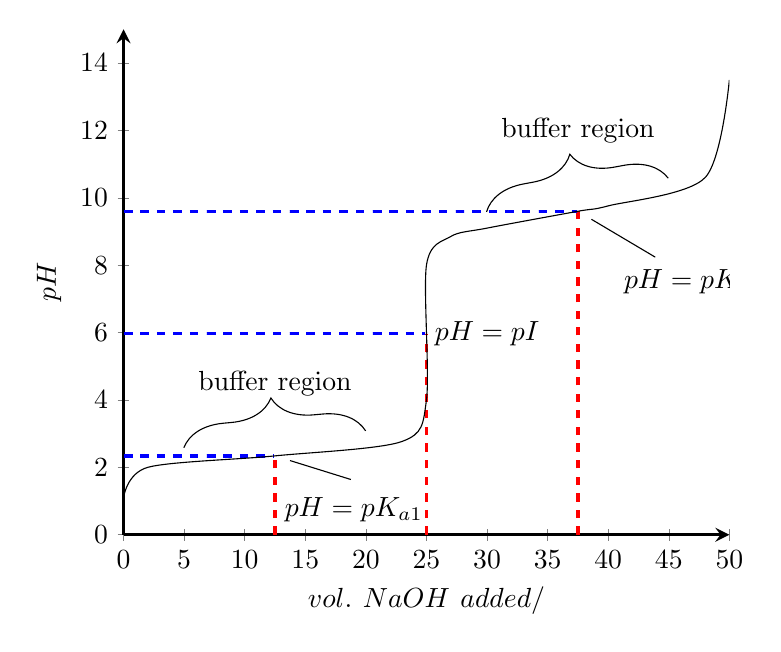
\begin{tikzpicture}

			\begin{axis}[
				axis lines		= left,
				domain			= 0:50,
				xlabel			= \textbf{$vol.\ NaOH\ added/\si{\cubic\centi\metre}$},
				ylabel			= \textbf{$pH$},
				axis line style	= very thick,
				height			= 80mm,
				samples			= 300,
				xtick			= {0, 5, 10, 15, 20, 25, 30, 35, 40, 45, 50}
			]

				% force the graph to show up to these
				\addplot[color = green, very thick, opacity = 0]{15};
				\addplot[color = green, very thick, opacity = 0]{0};

				\addplot[color = red, very thick, dashed] coordinates {(25, 0) (25, 5.97)};
				\addplot[color = blue, very thick, dashed, restrict x to domain = 0:25]{5.97};

				\addplot[color = red, very thick, dashed] coordinates {(12.5, 0) (12.5, 2.34)};
				\addplot[color = blue, very thick, dashed, restrict x to domain = 0:12.5]{2.34};

				\addplot[color = red, very thick, dashed] coordinates {(37.5, 0) (37.5, 9.60)};
				\addplot[color = blue, very thick, dashed, restrict x to domain = 0:37.5]{9.60};

				\draw[decorate, decoration={brace,amplitude=15pt,raise=1pt}] (5,2.5) -- (20,3.0);
				\node at (axis cs: 12.5,4.5) {buffer region};

				\draw[decorate, decoration={brace,amplitude=15pt,raise=1pt}] (30,9.5) -- (45,10.5);
				\node at (axis cs: 37.5,12.0) {buffer region};

				\draw[shorten <=2mm,shorten >=2mm] (12.5,2.34) -- (20,1.5);
				\node at (axis cs: 19,0.75) {$pH = pK_{a1}$};

				\node at (axis cs: 30,5.96) {$pH = pI$};

				\draw[shorten <=2mm,shorten >=2mm] (37.5,9.60) -- (45,8.0);
				\node at (axis cs: 47,7.5) {$pH = pK_{a2}$};



				% ORIGINAL DATASET:
				% (0,2.92) (1,3.47) (2,3.79) (3,3.98) (4,4.13) (5,4.25) (10,4.67) (15,5.03) (20,5.45) (21,5.57) (22,5.72)
				% (23,5.91) (24,6.23) (25,7.0) (25,8.78) (25,10.0) (26,11.29) (27,11.59) (28,11.75) (29,11.87) (30,11.96)
				% (35,12.22) (40,12.36) (45,12.46) (50,12.52)

				\addplot [color = black, mark = none, smooth] coordinates {
					(0,1.1) (2,2.0) (12.5,2.34) (23,2.77)
					(25,4.0) (25,8.0) (27,8.85) (30,9.1) (37.5,9.60) (40,9.76) (48,10.6) (50,13.5)
				};

			\end{axis}

		\end{tikzpicture}
		\end{center}

		The two \pKa{} values for glycine are, as can be guessed, \num{2.34} and \num{9.60}. These are the \pH{} levels where the carboxylic
		acid gets deprotonated, and where the amine gets deprotonated, respectively.

		At $pH = 2.34$, or $pK_{a1}$, the maximum buffer capacity is reached, and again at $pH = 9.60$, or $pK_{a2}$. When no \ch{NaOH} is
		added, the solution contains only the cationic form of the amino acid. When $pH = pI$, only the zwitterion exists in solution. When
		$pH > pK_{a2}$, only the anionic form exists.

	% end section

	\pagebreak
	\section{Peptide Bonds}

		Peptide bonds, or amide linkages, are the primary bonds holding amino acids together, allowing them to form longer, \itl{polypeptide}
		chains. A simple tripeptide, with two peptide bonds, looks like this:

		\diagram[1.0]{
			\chemfig{!\molRAmine-C(-[:90]H)(-[:270]!\molR)-C(=[:90]!\molO)-!\molN(-[:270]H)-C(-[:90]H)(-[:270]!\molR)-C(=[:90]!\molO)-!\molN(-[:270]H)-C(-[:90]H)(-[:270]!\molR)-C(=[:90]!\molO)(-[:0]!\molOH)}

			\chemmove{
				\draw[red,very thick] (-6,1.75) rectangle (-3.5,-1.5);
				\draw[red,very thick] (-9.5,1.75) rectangle (-7.25,-1.5);
			}
		}{The peptide linkages are boxed up in red.}


		\subsection{Peptide Bond Formation}

			Peptide bonds cannot actually be formed artificially, since the amine and the carboxylic acid will undergo an acid-base reaction
			instead of nucleophilic acyl substitution. A possible alternative is to use acyl chlorides.

			Biological things use enzymes to facilitate the creation of peptide bonds.

			The reaction is actually a condensation reaction, where a molecule of \ch{H2O} is eliminated to form the amide.

		% end subsection


		\subsection{Polypeptide Features}

			Polypeptides consist of a main \itl{backbone}, which is made up of a sequence of α-carbons followed by peptide bonds; R-groups
			are attached to this backbone.

			Since the constituent amino acids are no longer individually distinct, they are called \itl{amino acid residues}, since they
			can still be identified by the side-chain on the backbone.

			By convention, polypeptides are drawn with the \itl{N-terminus}, the open \ch{NH2} end, on the left, and the \itl{C-terminus},
			the open \ch{CO2H} end, on the right.

		% end subsection


		\subsection{Hydrolysis of Polypeptides}

			Under the right circumstances, polypeptide chains can be hydrolysed, although it takes a long time. Hydrolysis requires either
			an enzyme (pepsin), or a dilute acid or base, with heat. The heating needs to take place for \itl{several hours} to ensure
			complete hydrolysis.

			If there is incomplete hydrolysis, the reaction mixture might contain various amounts of single amino acids, dipeptides, tripeptides,
			and other things.

		% end subsection

	% end section

% end part













